

\documentclass{article}

% Recommended, but optional, packages for figures and better typesetting:
\usepackage{microtype}
\usepackage{graphicx}
\usepackage{subfigure}
\usepackage{booktabs} % for professional tables
\usepackage{lipsum}
% hyperref makes hyperlinks in the resulting PDF.
% If your build breaks (sometimes temporarily if a hyperlink spans a page)
% please comment out the following usepackage line and replace
% \usepackage{lfd2021} with \usepackage[nohyperref]{lfd2021} above.
\usepackage{hyperref}

% Attempt to make hyperref and algorithmic work together better:
\newcommand{\theHalgorithm}{\arabic{algorithm}}

% Use the following line for the initial blind version submitted for review:
\usepackage{lfd2021}
\icmltitlerunning{Report Template }

\begin{document}

\twocolumn[
\icmltitle{Learning from Data (Fall 2021)\\
Report Template }

\begin{icmlauthorlist}
\icmlauthor{Alice Zhang}{to}
\icmlauthor{Bob Chen}{to}
\end{icmlauthorlist}

\icmlaffiliation{to}{Data Science and Information Technology Research Center, Tsinghua-Berkeley Shenzhen Institute, Tsinghua University, China}


\vskip 0.3in
]

\printAffiliationsAndNotice{} % otherwise use the standard text.


\begin{abstract}
\lipsum[1]
\end{abstract}

\section{Introduction}
\label{intro}
% use "figure*" instead of "feature" to display wide figure 
\begin{figure*}[t]
\vskip 0.2in
\begin{center}
\centerline{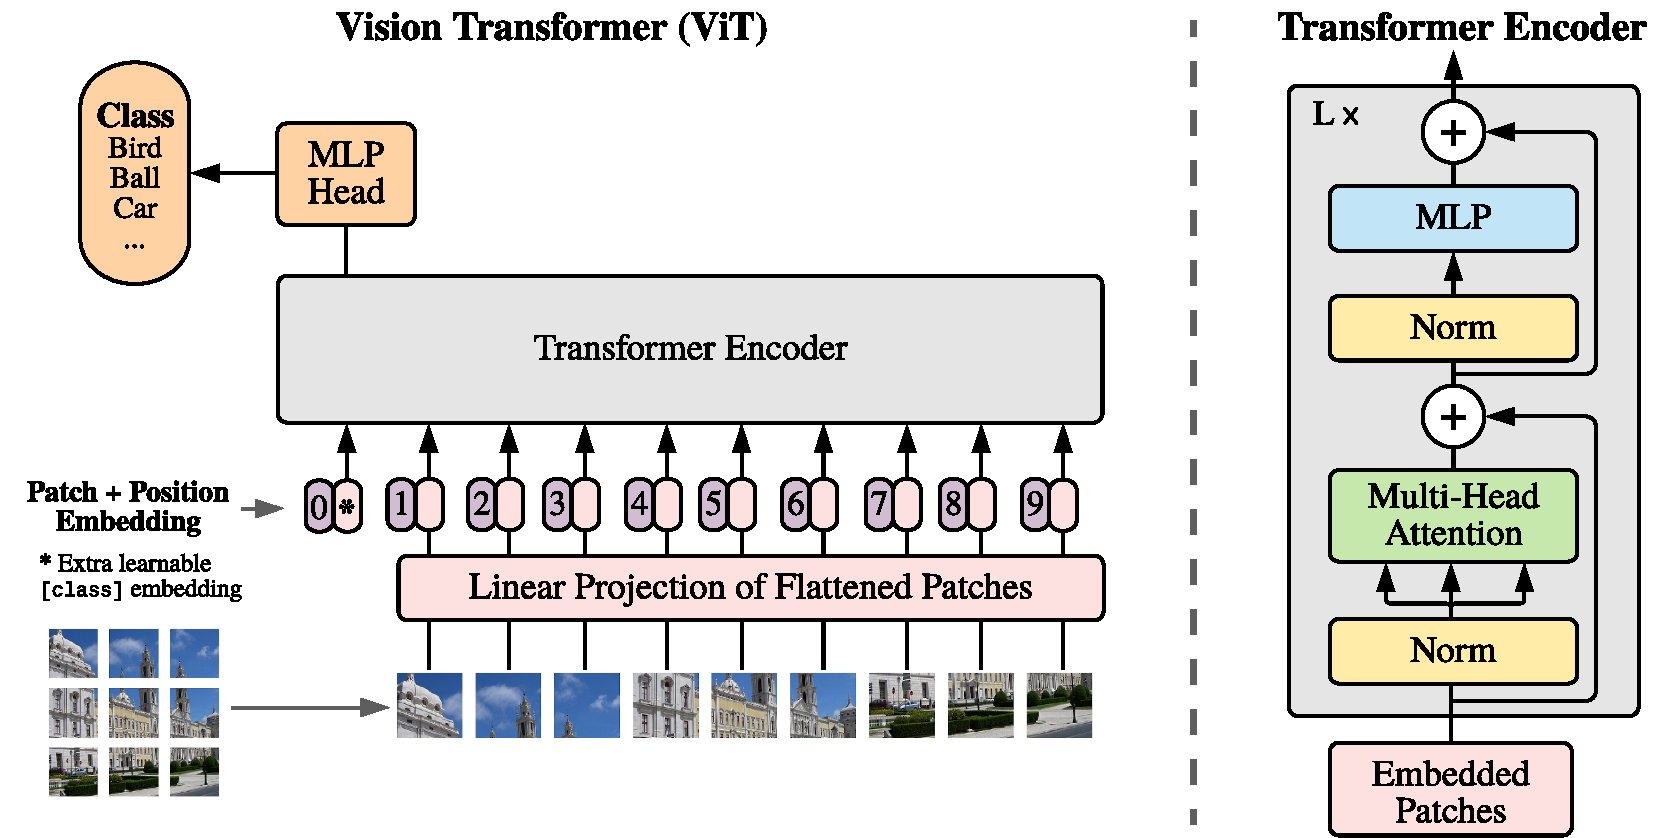
\includegraphics[width=\textwidth]{img/model_scheme.pdf}}
\caption{Display wide figure in two-column template.}
\label{model_overview}
\end{center}
\vskip -0.2in
\end{figure*}

\lipsum[2]

\lipsum[3]

In summary, the technical contributions include:

\begin{itemize}
\item Contribution 1.
\item Contribution 2.
\item Contribution 3.
\end{itemize}

\section{Related Work}

\textbf{Research field 1: }Transformer 
\cite{imagenet_cvpr09,vaswani2017attention} were proposed for machine translation, and have since become the state of the art method in many NLP tasks. \lipsum[4]

\textbf{Research field 2: }\lipsum[5]

\section{Method}

\lipsum[6]

\subsection{Part 1}
\lipsum[7-9] See algorithm~\ref{alg:example}.

\begin{algorithm}[tb]
   \caption{Bubble Sort}
   \label{alg:example}
\begin{algorithmic}
   \STATE {\bfseries Input:} data $x_i$, size $m$
   \REPEAT
   \STATE Initialize $noChange = true$.
   \FOR{$i=1$ {\bfseries to} $m-1$}
   \IF{$x_i > x_{i+1}$}
   \STATE Swap $x_i$ and $x_{i+1}$
   \STATE $noChange = false$
   \ENDIF
   \ENDFOR
   \UNTIL{$noChange$ is $true$}
\end{algorithmic}
\end{algorithm}

\subsection{Part 2}
\lipsum[10-12]

\section{Results}

\lipsum[13]

\begin{figure}[ht]
\vskip 0.2in
\begin{center}
\centerline{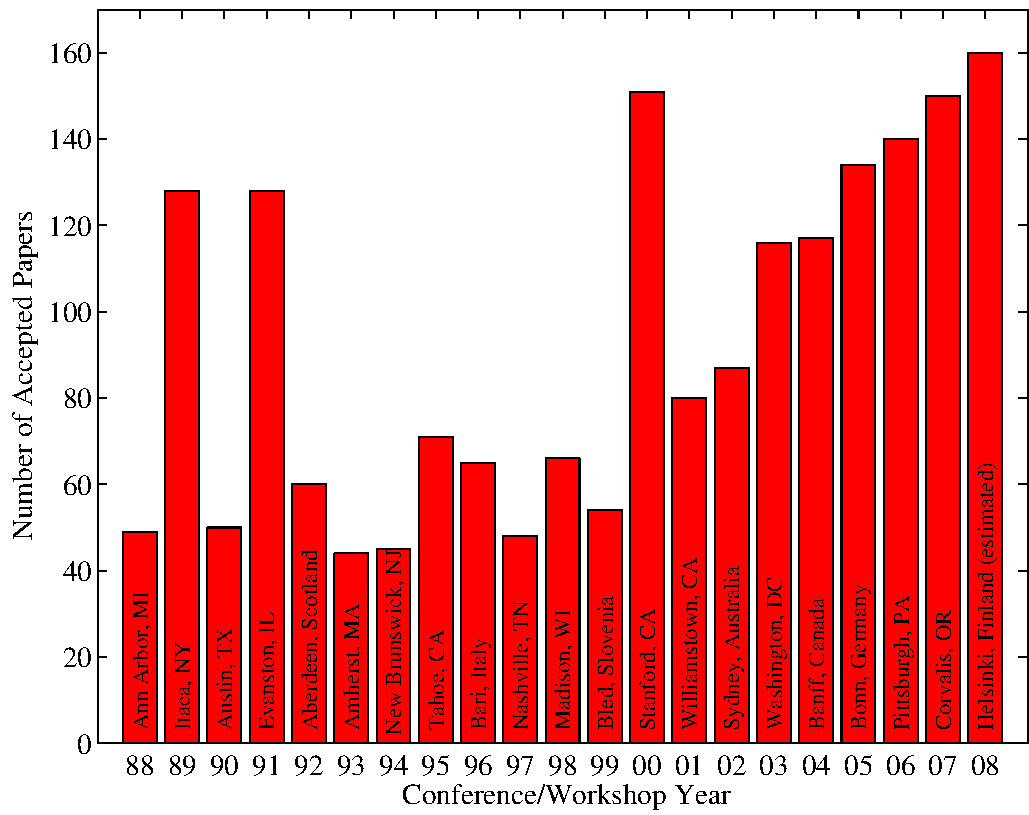
\includegraphics[width=\columnwidth]{img/icml_numpapers}}
\caption{Display figure in column.}
\label{icml-historical}
\end{center}
\vskip -0.2in
\end{figure}

\lipsum[14]

\begin{table}[t]
\caption{Display table in column.}
\label{sample-table}
\vskip 0.15in
\begin{center}

\begin{tabular}{lcccr}
\toprule
Data set & Naive & Flexible & Better? \\
\midrule
Breast   & 95.9$\pm$ 0.2& 96.7$\pm$ 0.2& $\surd$ \\
Cleveland & 83.3$\pm$ 0.6& 80.0$\pm$ 0.6& $\times$\\
Glass2    & 61.9$\pm$ 1.4& 83.8$\pm$ 0.7& $\surd$ \\
Credit    & 74.8$\pm$ 0.5& 78.3$\pm$ 0.6&         \\
Horse     & 73.3$\pm$ 0.9& 69.7$\pm$ 1.0& $\times$\\
Meta      & 67.1$\pm$ 0.6& 76.5$\pm$ 0.5& $\surd$ \\
Pima      & 75.1$\pm$ 0.6& 73.9$\pm$ 0.5&         \\
Vehicle   & 44.9$\pm$ 0.6& 61.5$\pm$ 0.4& $\surd$ \\
\bottomrule
\end{tabular}
\end{center}
\vskip -0.1in
\end{table}


\begin{table*}[t]
\caption{Wide table in two-column template.}
\centering
\resizebox{1.98\columnwidth}{!}{
\begin{tabular}{lrrrrr}
\toprule
\multicolumn{1}{c}{Classifier} & \multicolumn{1}{c}{Identity Accuracy} & \multicolumn{1}{c}{Human-Agent Accuracy} & \multicolumn{1}{c}{Human-Agent Rank} & \multicolumn{1}{c}{Hybrid-Symbolic Accuracy} & \multicolumn{1}{c}{Hybrid-Symbolic Rank} \\
\midrule
SYM-FF & $0.850$ $(0.062)$ & $0.850$ $(0.062)$ & $0.364$ $(0.043)$ & $0.475$ $(0.166)$ & $-0.244$ $(0.252)$ \\
SYM-GRU & $0.850$ $(0.082)$ & $0.850$ $(0.082)$ & $0.173$ $(0.049)$ & $0.400$ $(0.200)$ & $-0.249$ $(0.210)$ \\
\midrule
VIS-FF  & $0.633$ $(0.041)$ & $0.633$ $(0.041)$ & $-0.041$ $(0.160)$ & $0.225$ $(0.050)$ & $-0.165$ $(0.286)$ \\
VIS-GRU & $0.767$ $(0.097)$ & $0.767$ $(0.097)$ & $0.220$ $(0.267)$ & $0.425$ $(0.127)$ & $-0.056$ $(0.331)$ \\
\midrule
TD-CNN & $0.583$ $(0.075)$ & $0.583$ $(0.075)$ & $0.222$ $(0.059)$ & $0.525$ $(0.094)$ & $-0.093$ $(0.149)$ \\
BC-CNN & $0.717$ $(0.145)$ & $0.717$ $(0.145)$ & $-0.009$ $(0.131)$ & $0.475$ $(0.050)$ & $-0.095$ $(0.412)$ \\
\bottomrule
\end{tabular}
}% end resizebox
\vskip -.2cm
\label{table:results-classifiers}
\vskip -.1cm
\end{table*}

\lipsum[11]



\section{Conclusions \& Discussion}

\lipsum[10]

\section{Author Contribution \& Acknowledgement}
Alice built the model and ran experiments. Bob  carried 
  out analyses. Bob and Alice wrote and edited the report. We thank Charlie from the Delta Lab for providing the data and technical support.  


% In the unusual situation where you want a paper to appear in the
% references without citing it in the main text, use \nocite

\nocite{dosovitskiy2020image}

\bibliographystyle{lfd2021}
\bibliography{ref}

\end{document}
